\chapter{The \texorpdfstring{$P(3, -3, n)$}{P(3, -3, n)} family}
\section{Motivation}
In the case of Legendrian knots it is clear that ribbon knots can be constructed from a sufficiently stabilized unknot using the Reidemeister moves, one 0-handle, and one 1-handle. 
Starting from the unknot, we add a second unknot with a zero-handle, and then use Legendrian isotopy to "pass" the tip of the first unknot through the two loops as desired, before finally using a 1-handle to join the ribbon tip to the second unknot, thus closing the knot. 

The cobordism created by these moves is necessarily a concordance: The surfaces corresponding to each unknot have genus zero before the addition of the 1-handle, which connects them in only one place. In a constructible cobordism, genus can only be created by a 1-handle between connected components.

Thus to construct such a cobordism to a ribbon knot $K$, we have to start with an unknot $U$ with $\tb U = \tb K$. Given the topological knot type of $K$, the unknot and $K$ must certainly have $\tb \leq \overline{\tb} K$.
It is an open question when this can be achieved with equality: that is, when a cobordism can be constructed from a stabilized unknot to a maximal-$\tb$ Legendrian ribbon knot.

\section{Introduction of Result}
The main result of this project is the demonstration of a family of ribbon knots for which such a cobordism may be constructed with maximal Thurston-Bennequin number.

\begin{theorem}\label{thm:mine}
    Let $P_n = P(3, -3, n)$, for $n$ an integer. Then there exists a constructable Lagrangian concordance from an unknot $U$ with $\tb U = \maxtb P_n$ to a Legendrian representative of $P_n$.
\end{theorem}

\begin{figure}[ht!]
    \centering
    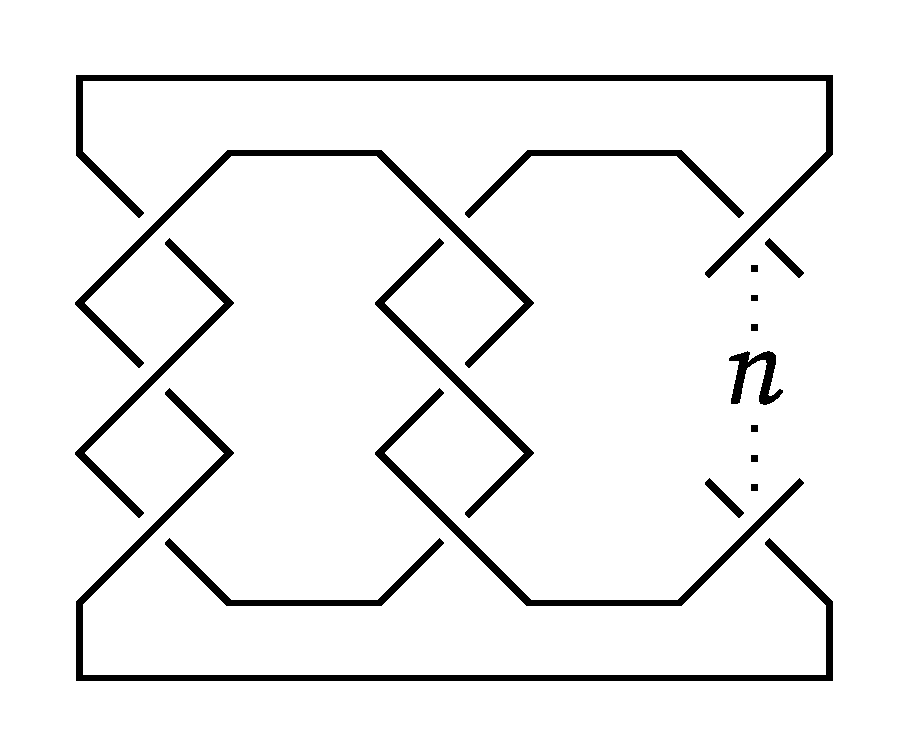
\includegraphics[width=0.4\textwidth]{images/pretzel-knot.pdf}
    \label{fig:pretzel-knot}
    \caption{The pretzel knot $P(3, -3, n)$. On the right, there are $n$ right half-twists (left half-twists for negative $n$).}
\end{figure}

For example, $P(3, -3, 0) = 3_1 \# m(3_1)$. Further, $P_1 = 6_1$; $P_2 = 8_{20}$; $P_3 = 9_{46}$; and $P_4 = 10_{140}$. Further note that $P_n = m(P_{-n})$ \cite{kawauchi}.

We sketch the construction used in the proof of Theorem \ref{thm:mine}. First, we make use of \cite{lu-zhong} to compute the Kauffman polynomial of $P(3, -3, n)$. From this we can obtain the Kauffman bound : it is $\maxtb{P_n} \leq \text{min}(-1, n-4)$. By Ng \cite{ng}, the Kauffman bound is sharp for $P_n$ (with the exception of $P_2$, but it is known that $\maxtb P_2 = -2$ and $\maxtb P_{-2} = -6$. This information is readily available in the Legendrian knot atlas\cite{atlas}.) and so $\maxtb P_n = \text{min} (-1, n-4)$.

With the desired $\tb$ in hand, we construct a suitable unknot according to $n$. We will use a combination of stabilization and $r_1$ moves to add a total of $n-1$ half-twists. There are three cases.
\pagebreak
\begin{itemize}

    \item[$n \leq 0$ :]
        The desired $\tb$ is $n-4$. We start with an unknot as seen below, with $n-1$ half-twists. Pictured here is $P_{-2}$, with 3 left half-twists.
        \begin{figure}[h!]
            \centering
            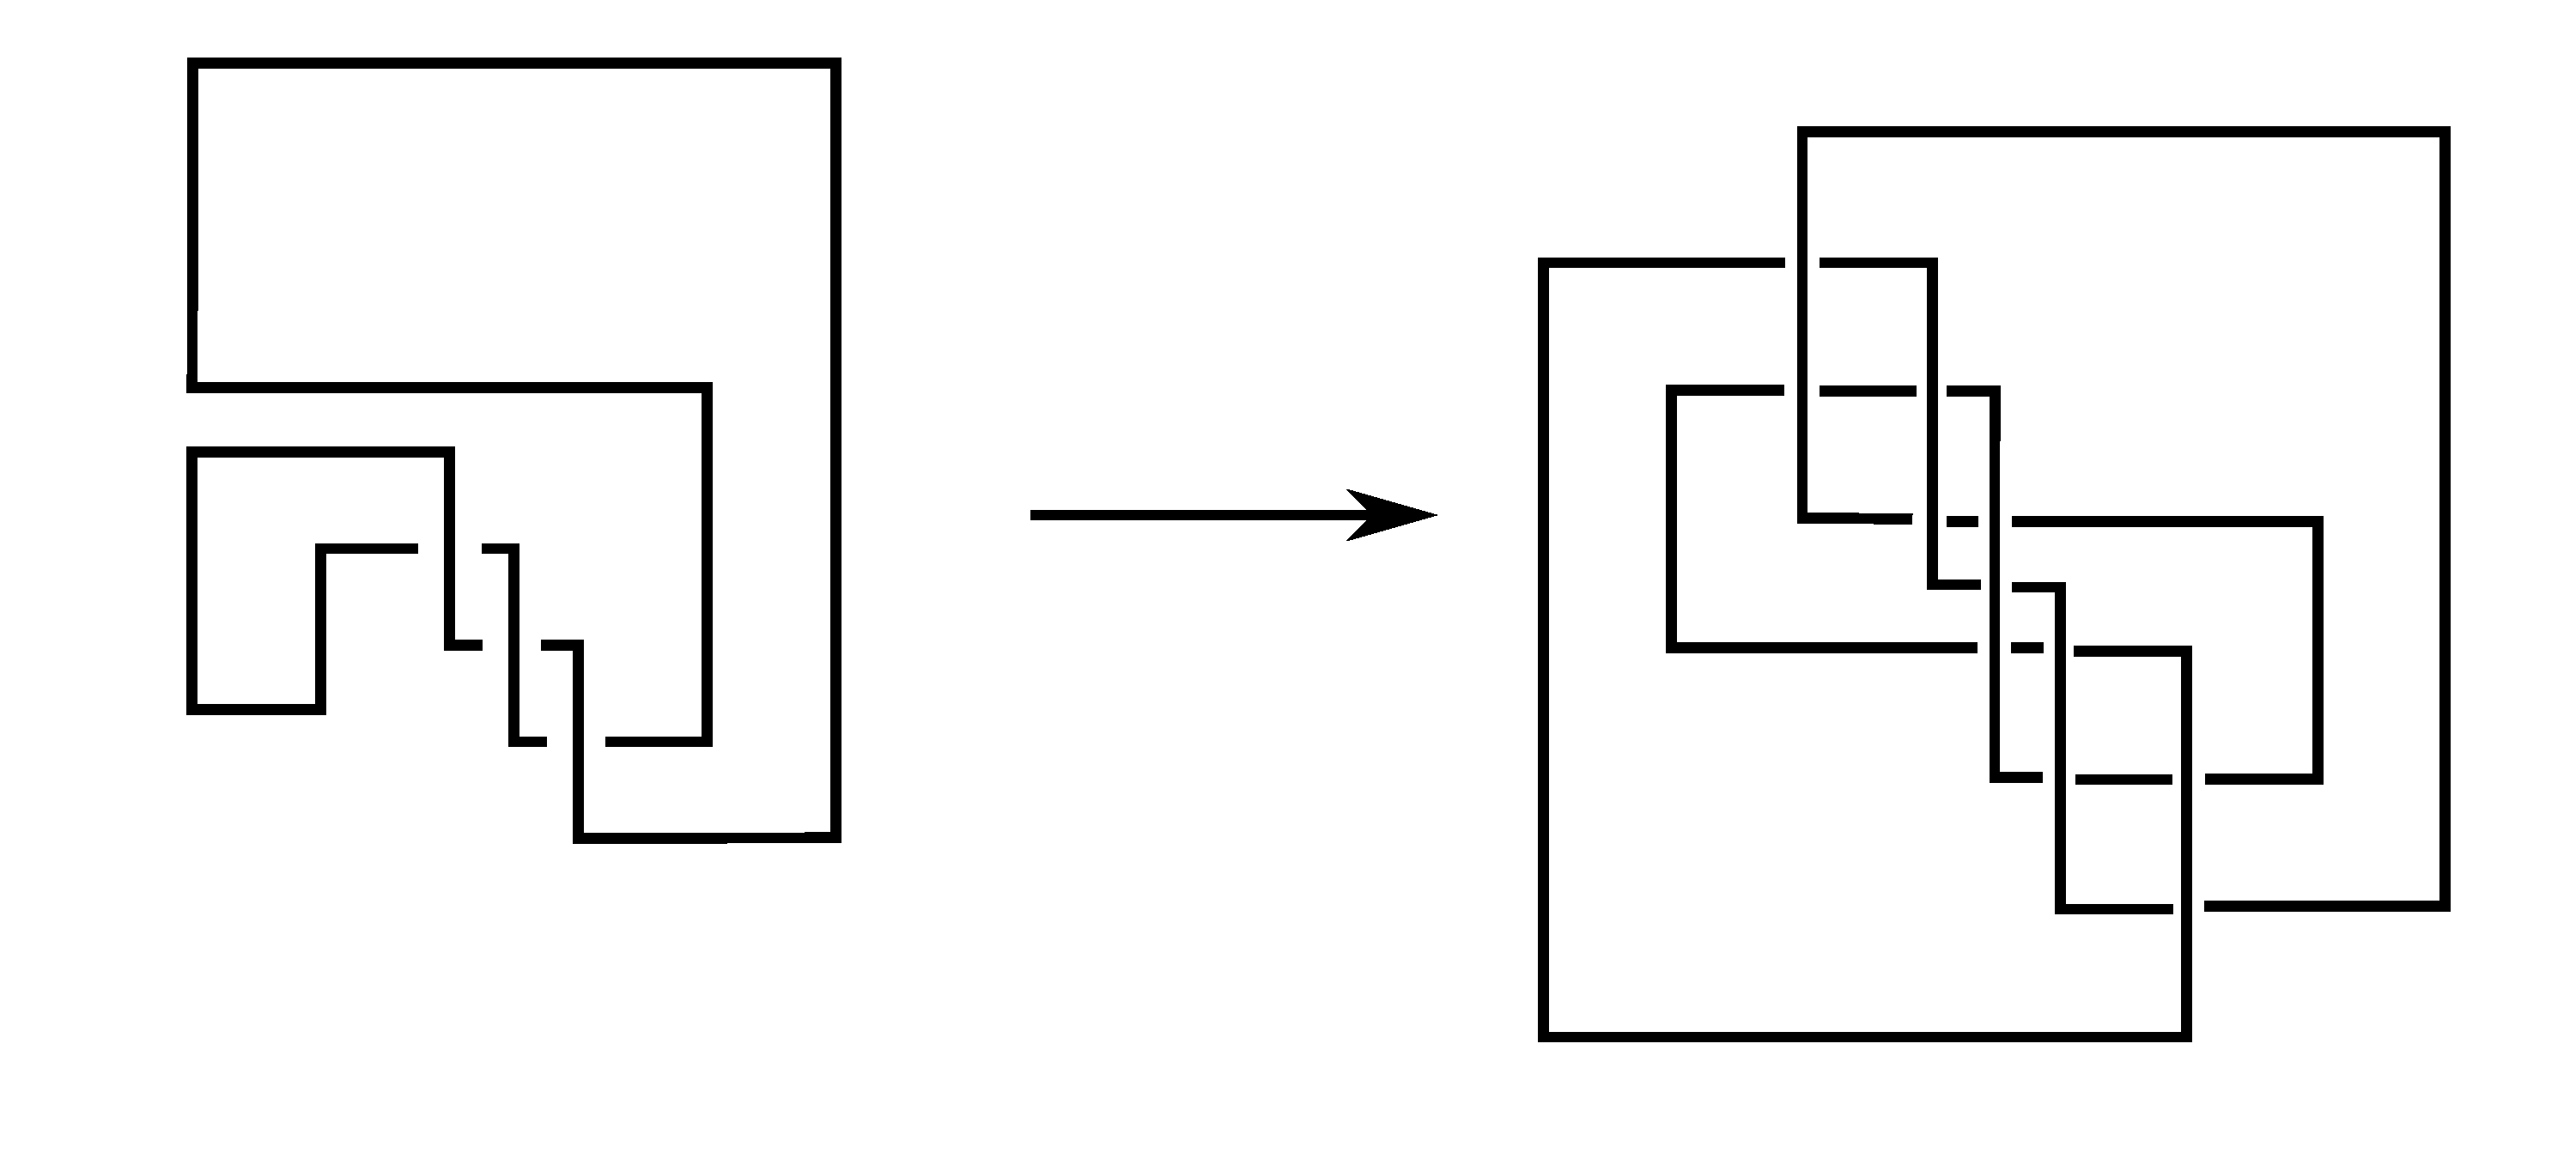
\includegraphics[width=0.4\textwidth]{images/pretzel--2-construction.pdf}
            \label{fig:pretzel-2}
            \caption{Unknot and resulting diagram for $P_{-2}$.}
        \end{figure}

    \item[$1 \leq n \leq 3$ :]
        Depending on $n$ this is $6_1$, $8_{20}$, or $9_{46}$. Each has a slightly different placement of twists.
        \begin{figure}[h!]
            \centering
            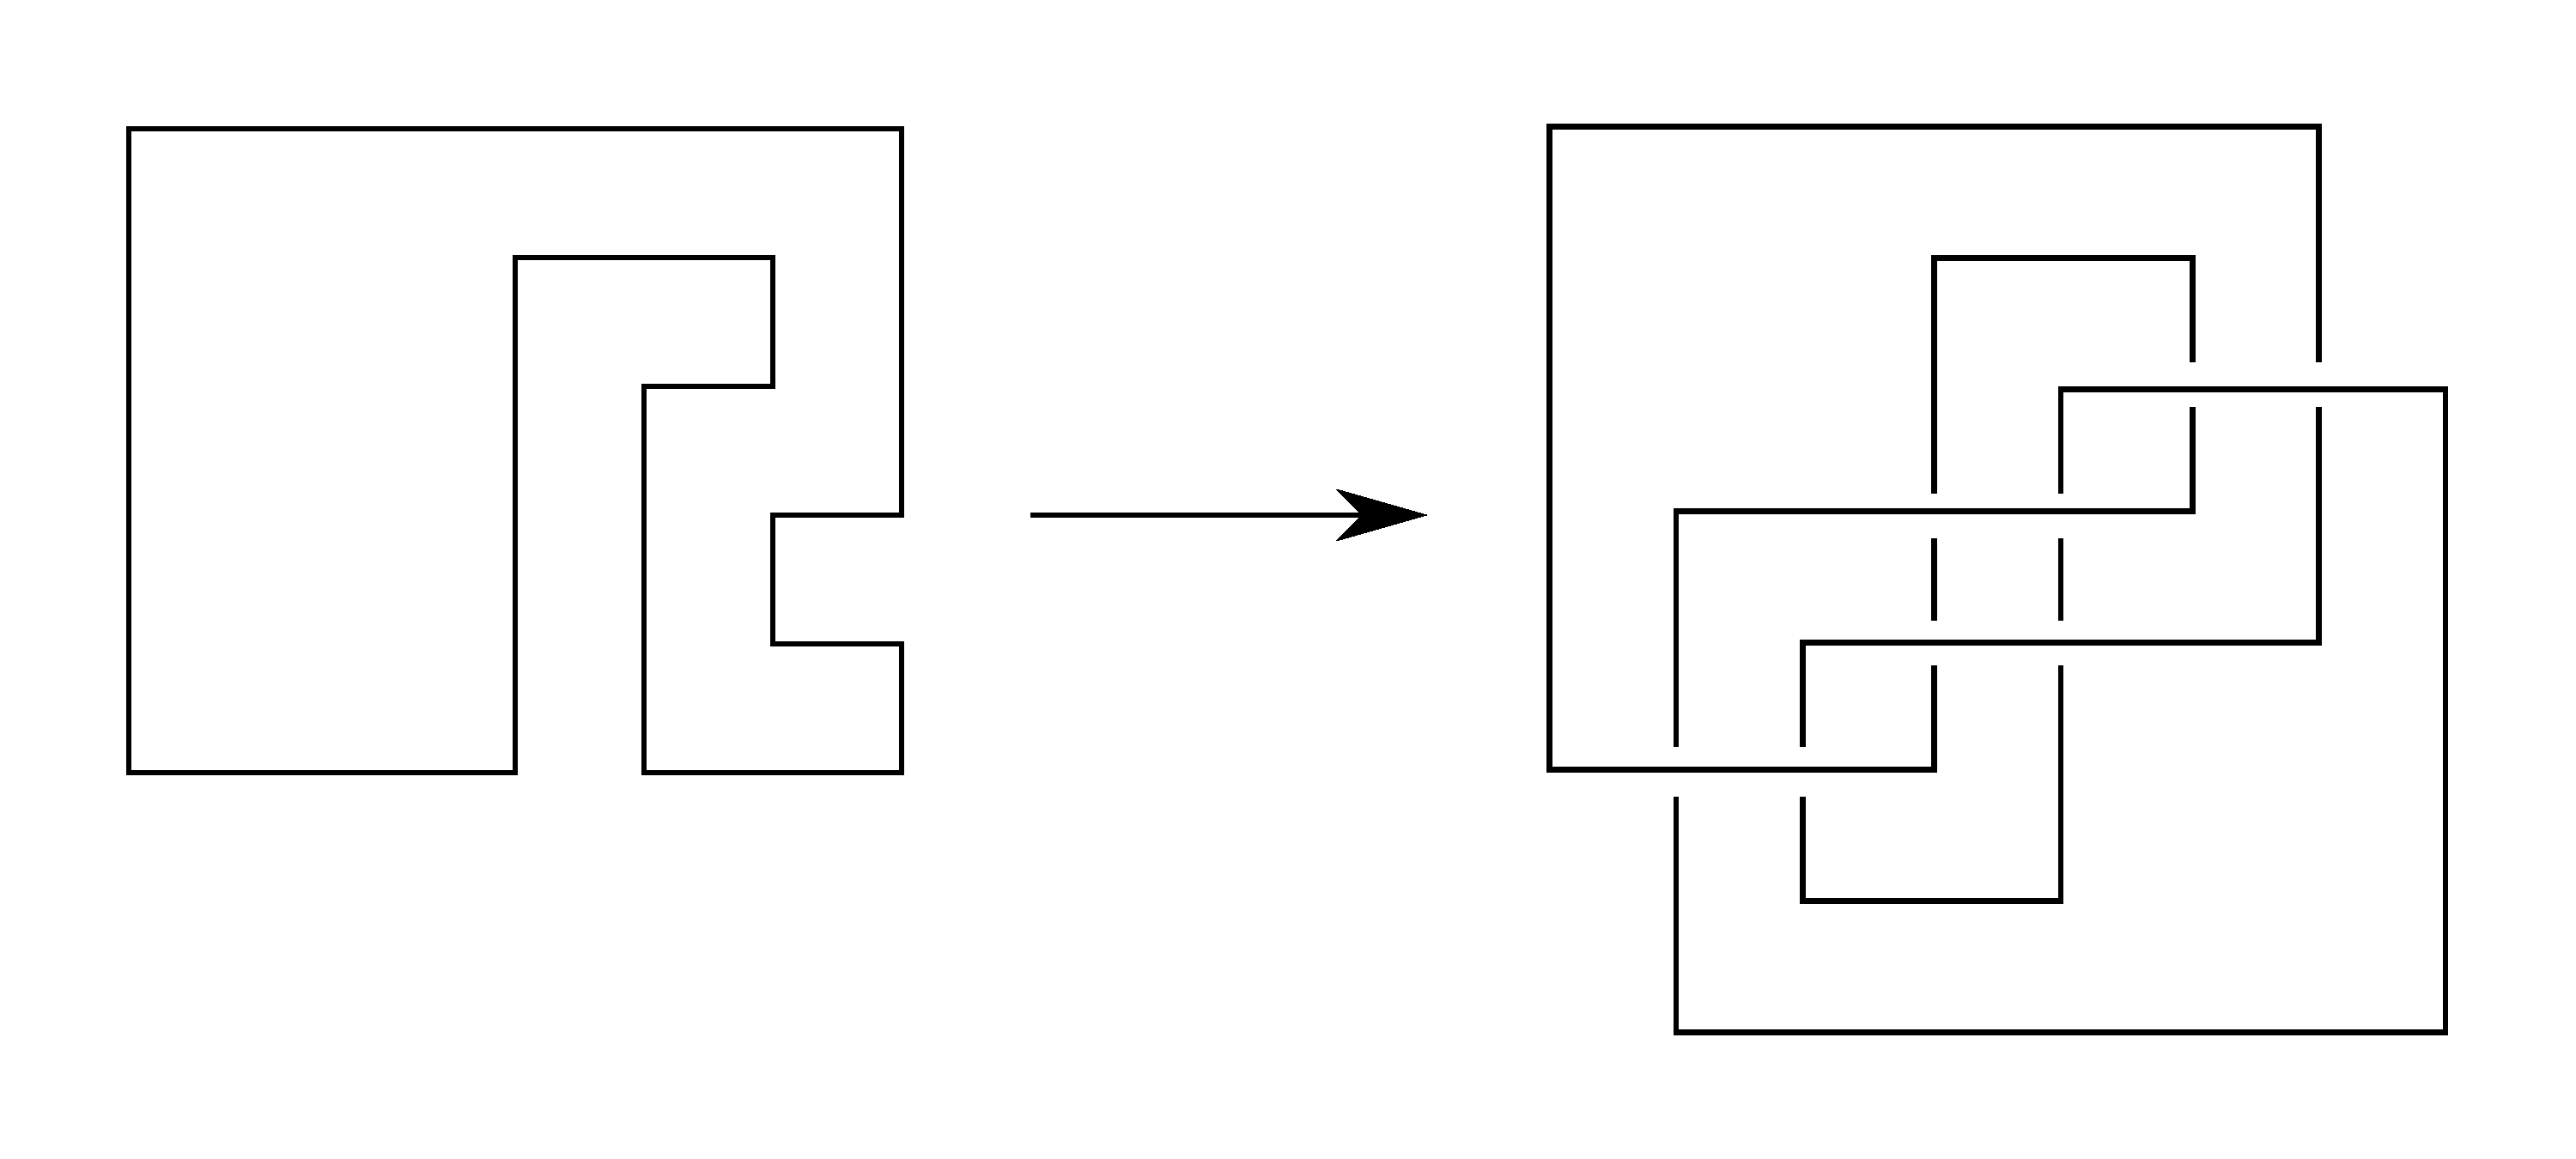
\includegraphics[width=0.3\textwidth]{images/pretzel-+1-construction.pdf} \hfill
            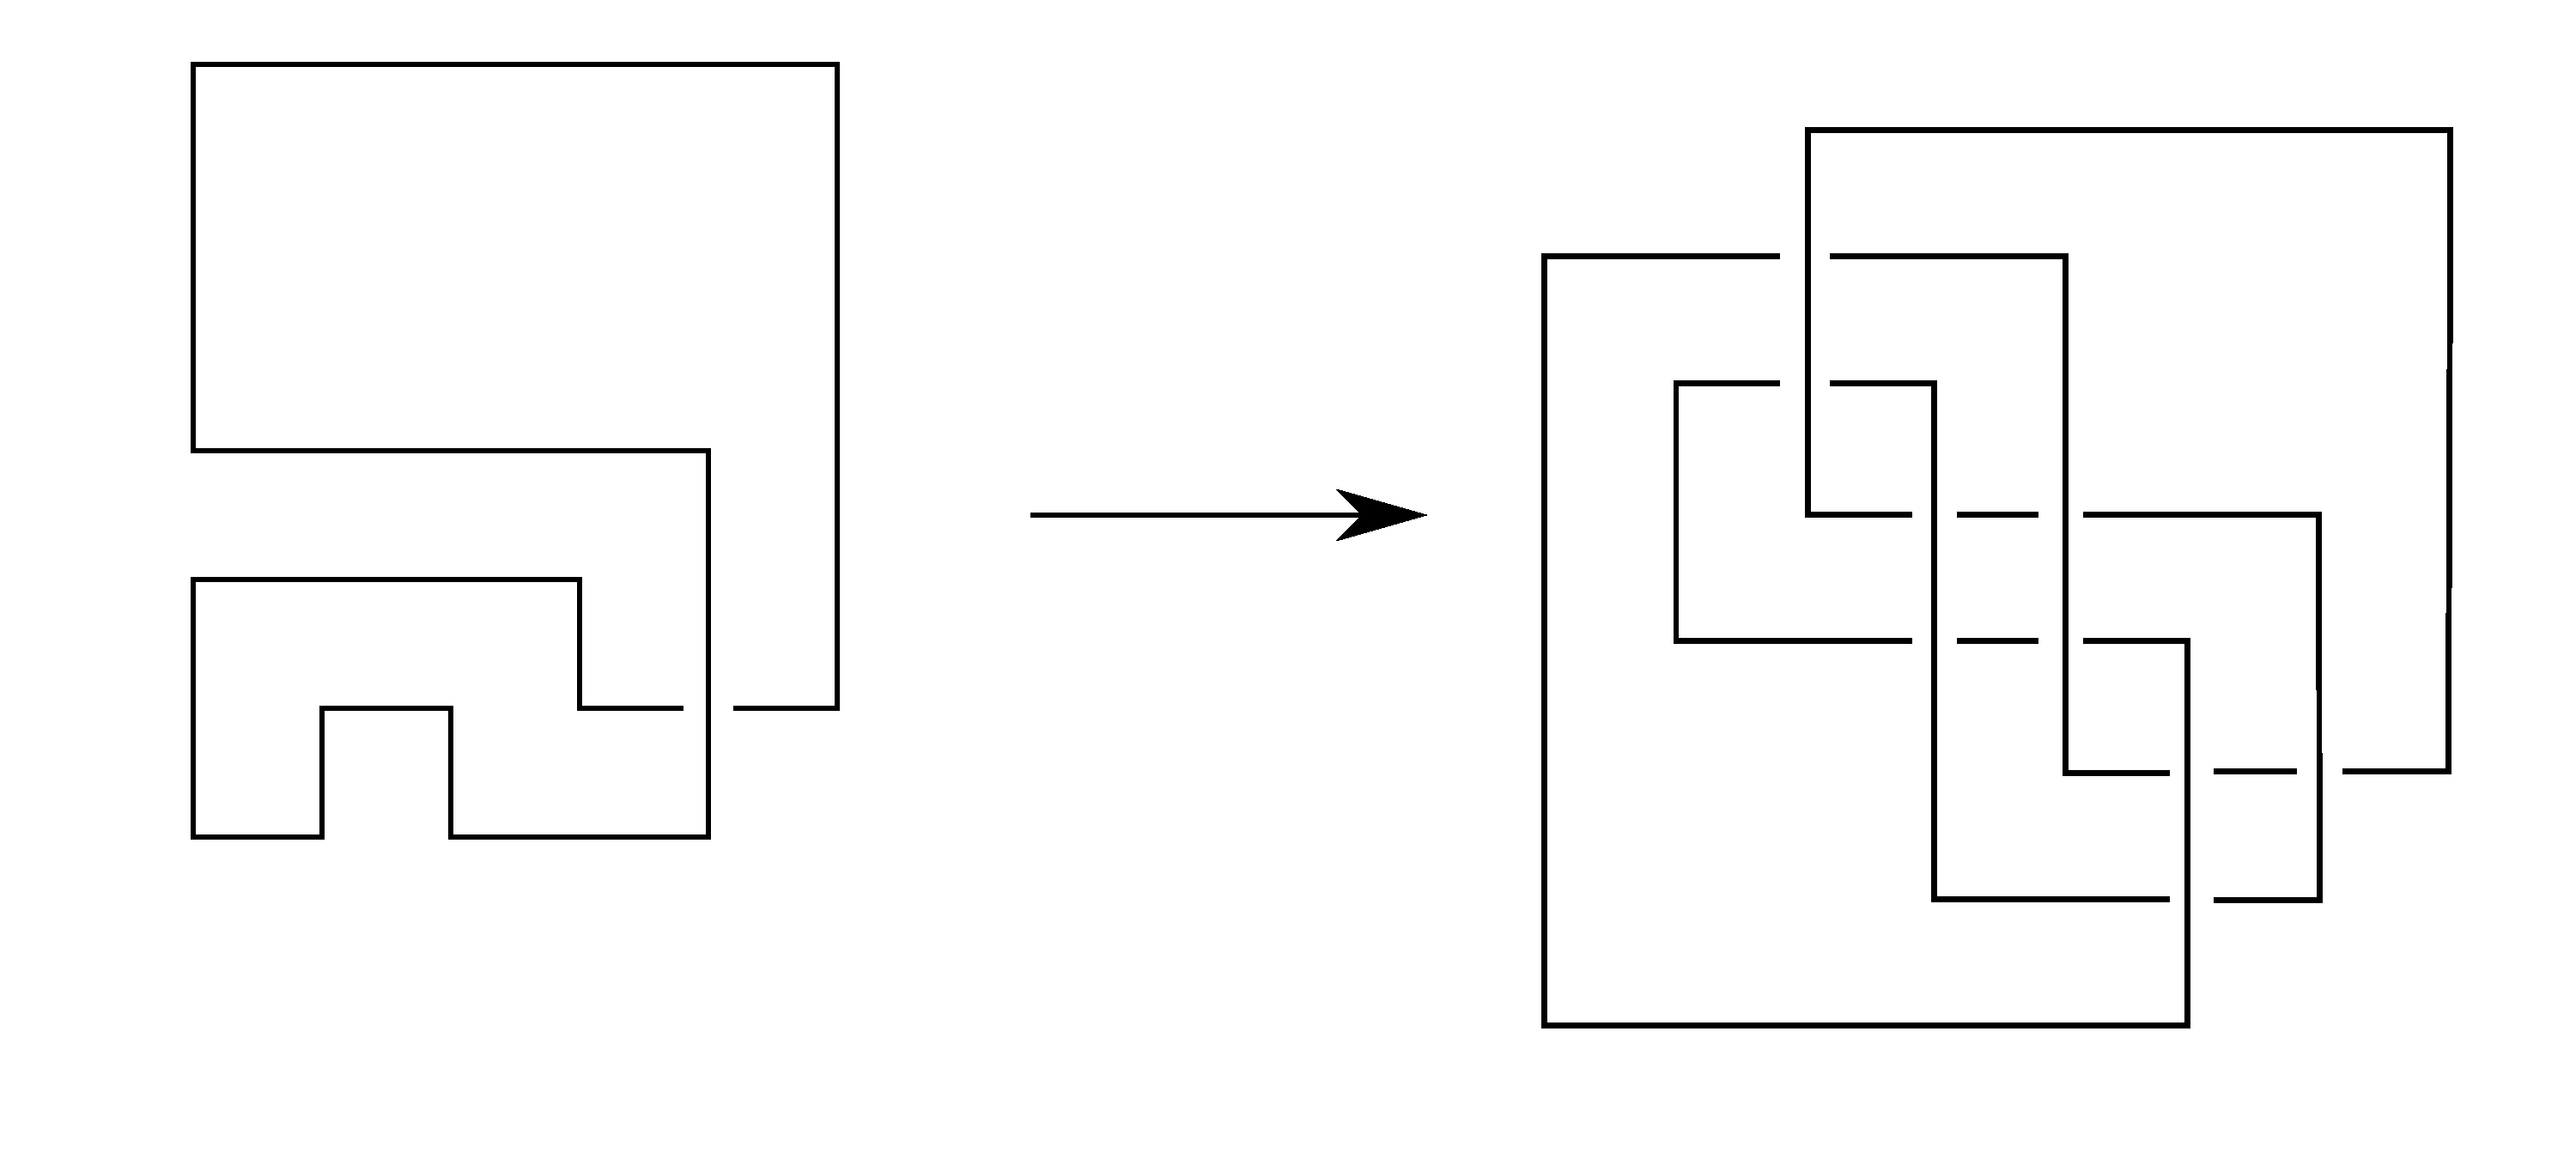
\includegraphics[width=0.3\textwidth]{images/pretzel-+2-construction.pdf} \hfill
            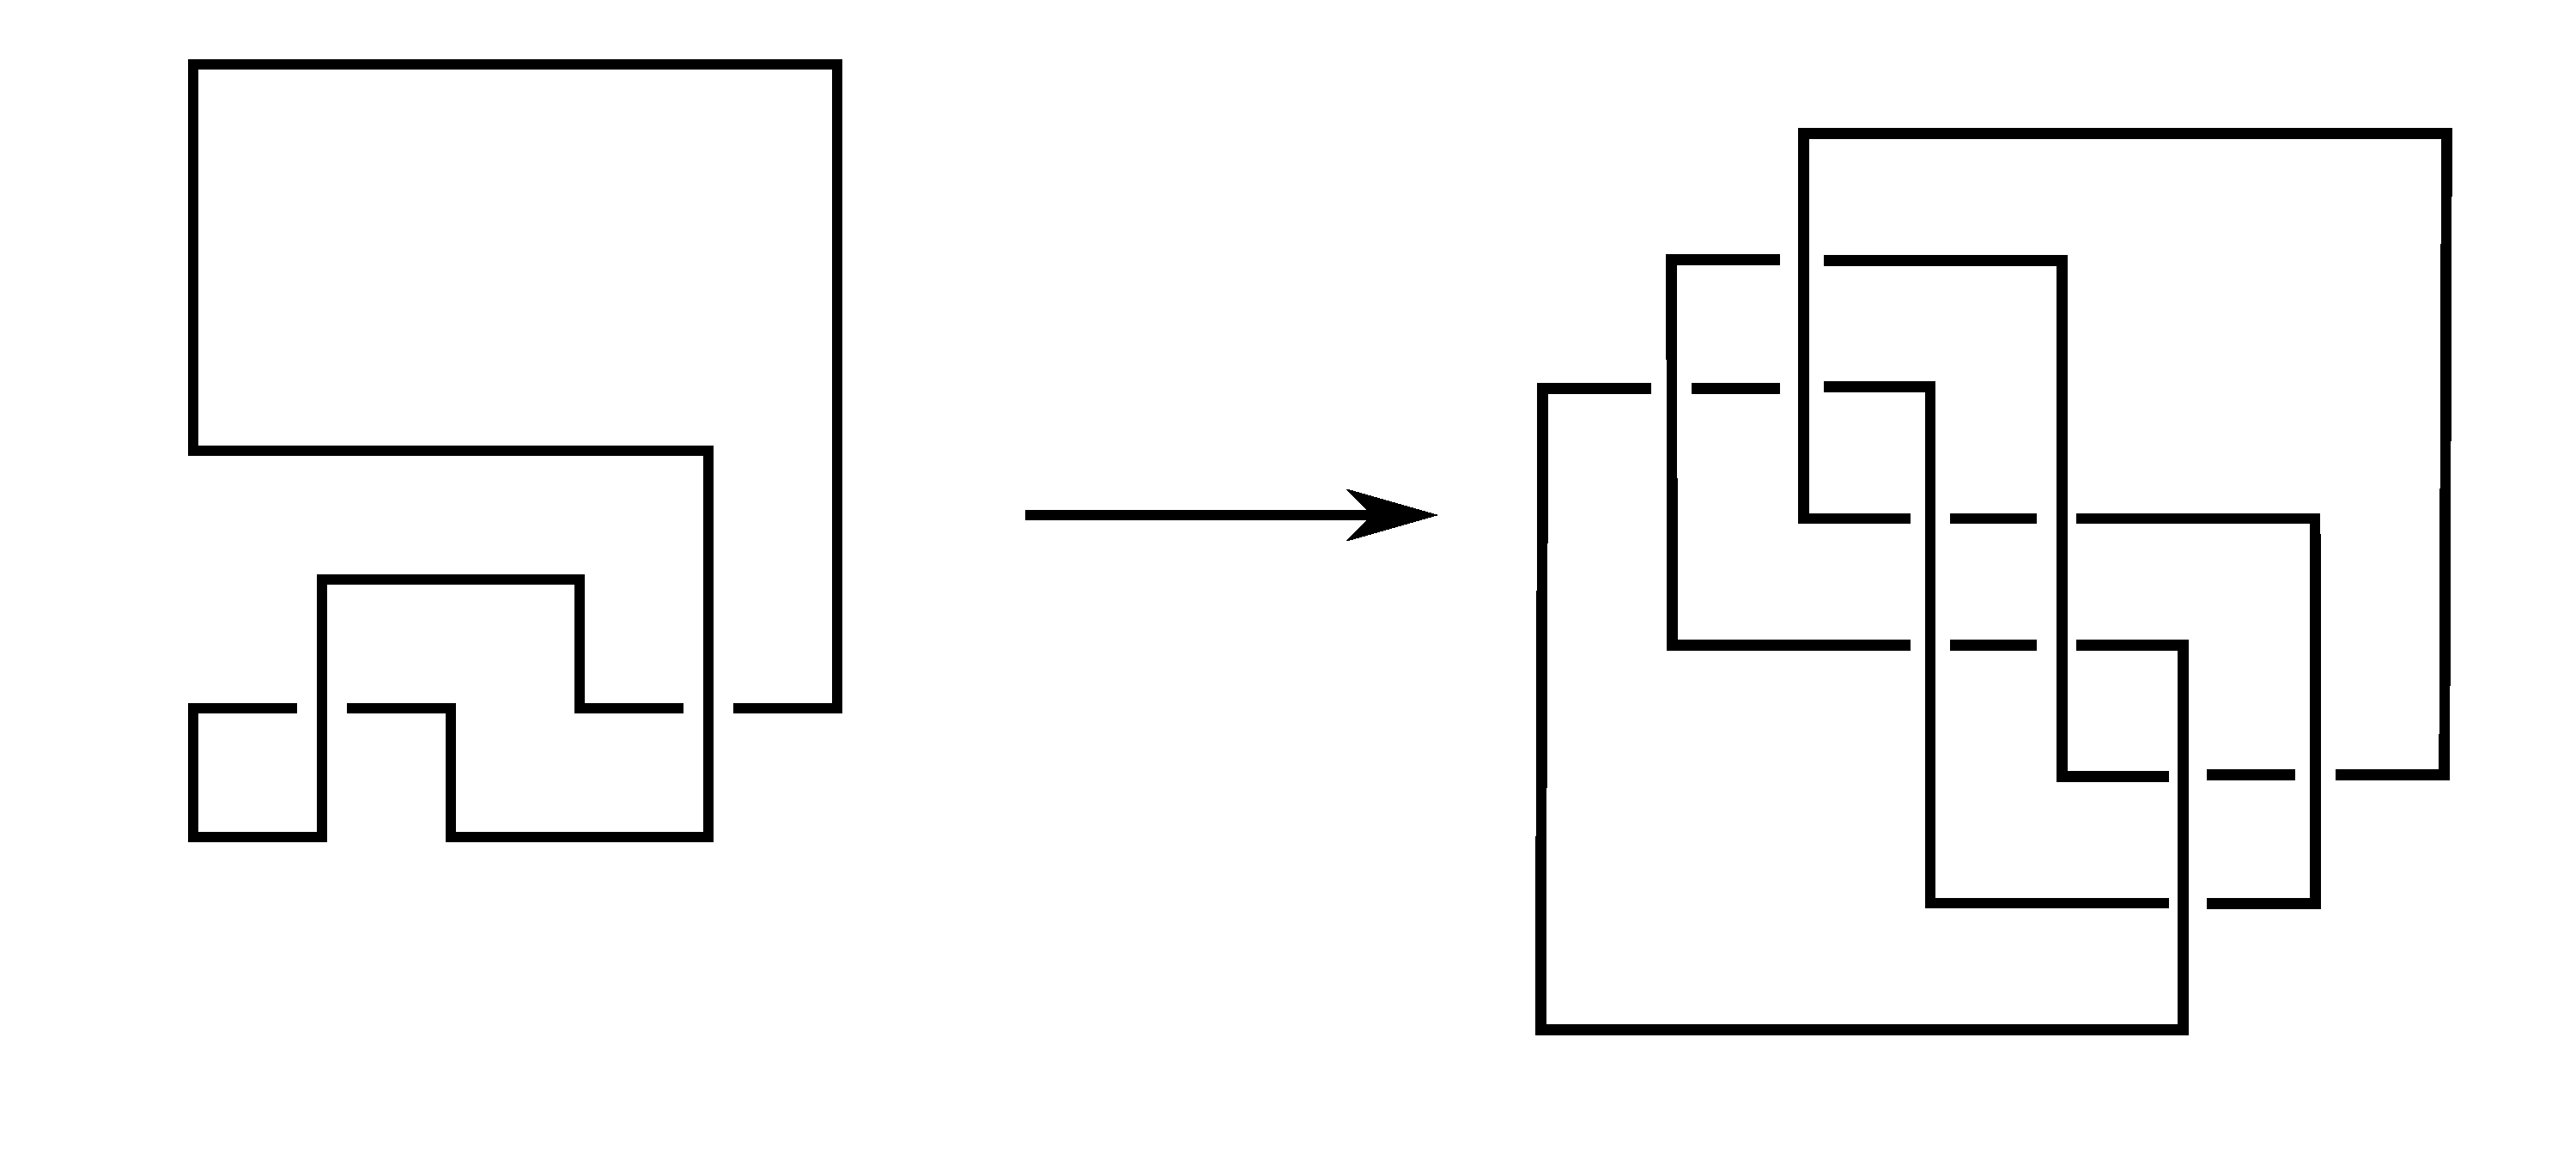
\includegraphics[width=0.3\textwidth]{images/pretzel-+3-construction.pdf}
            \label{fig:pretzel-singles}
            \caption{Unknots and resulting diagrams for $P_1$, $P_2$, and $P_3$ respectively.}
        \end{figure}

    \item[$n \geq 4$ :]
        The desired $tb$ is $-1$. Using the $r_1$ move we can add as many half-twists as we like (ie, $n - 1$) to our unknot before we make the pinch move.
        \begin{figure}[h!]
            \centering
            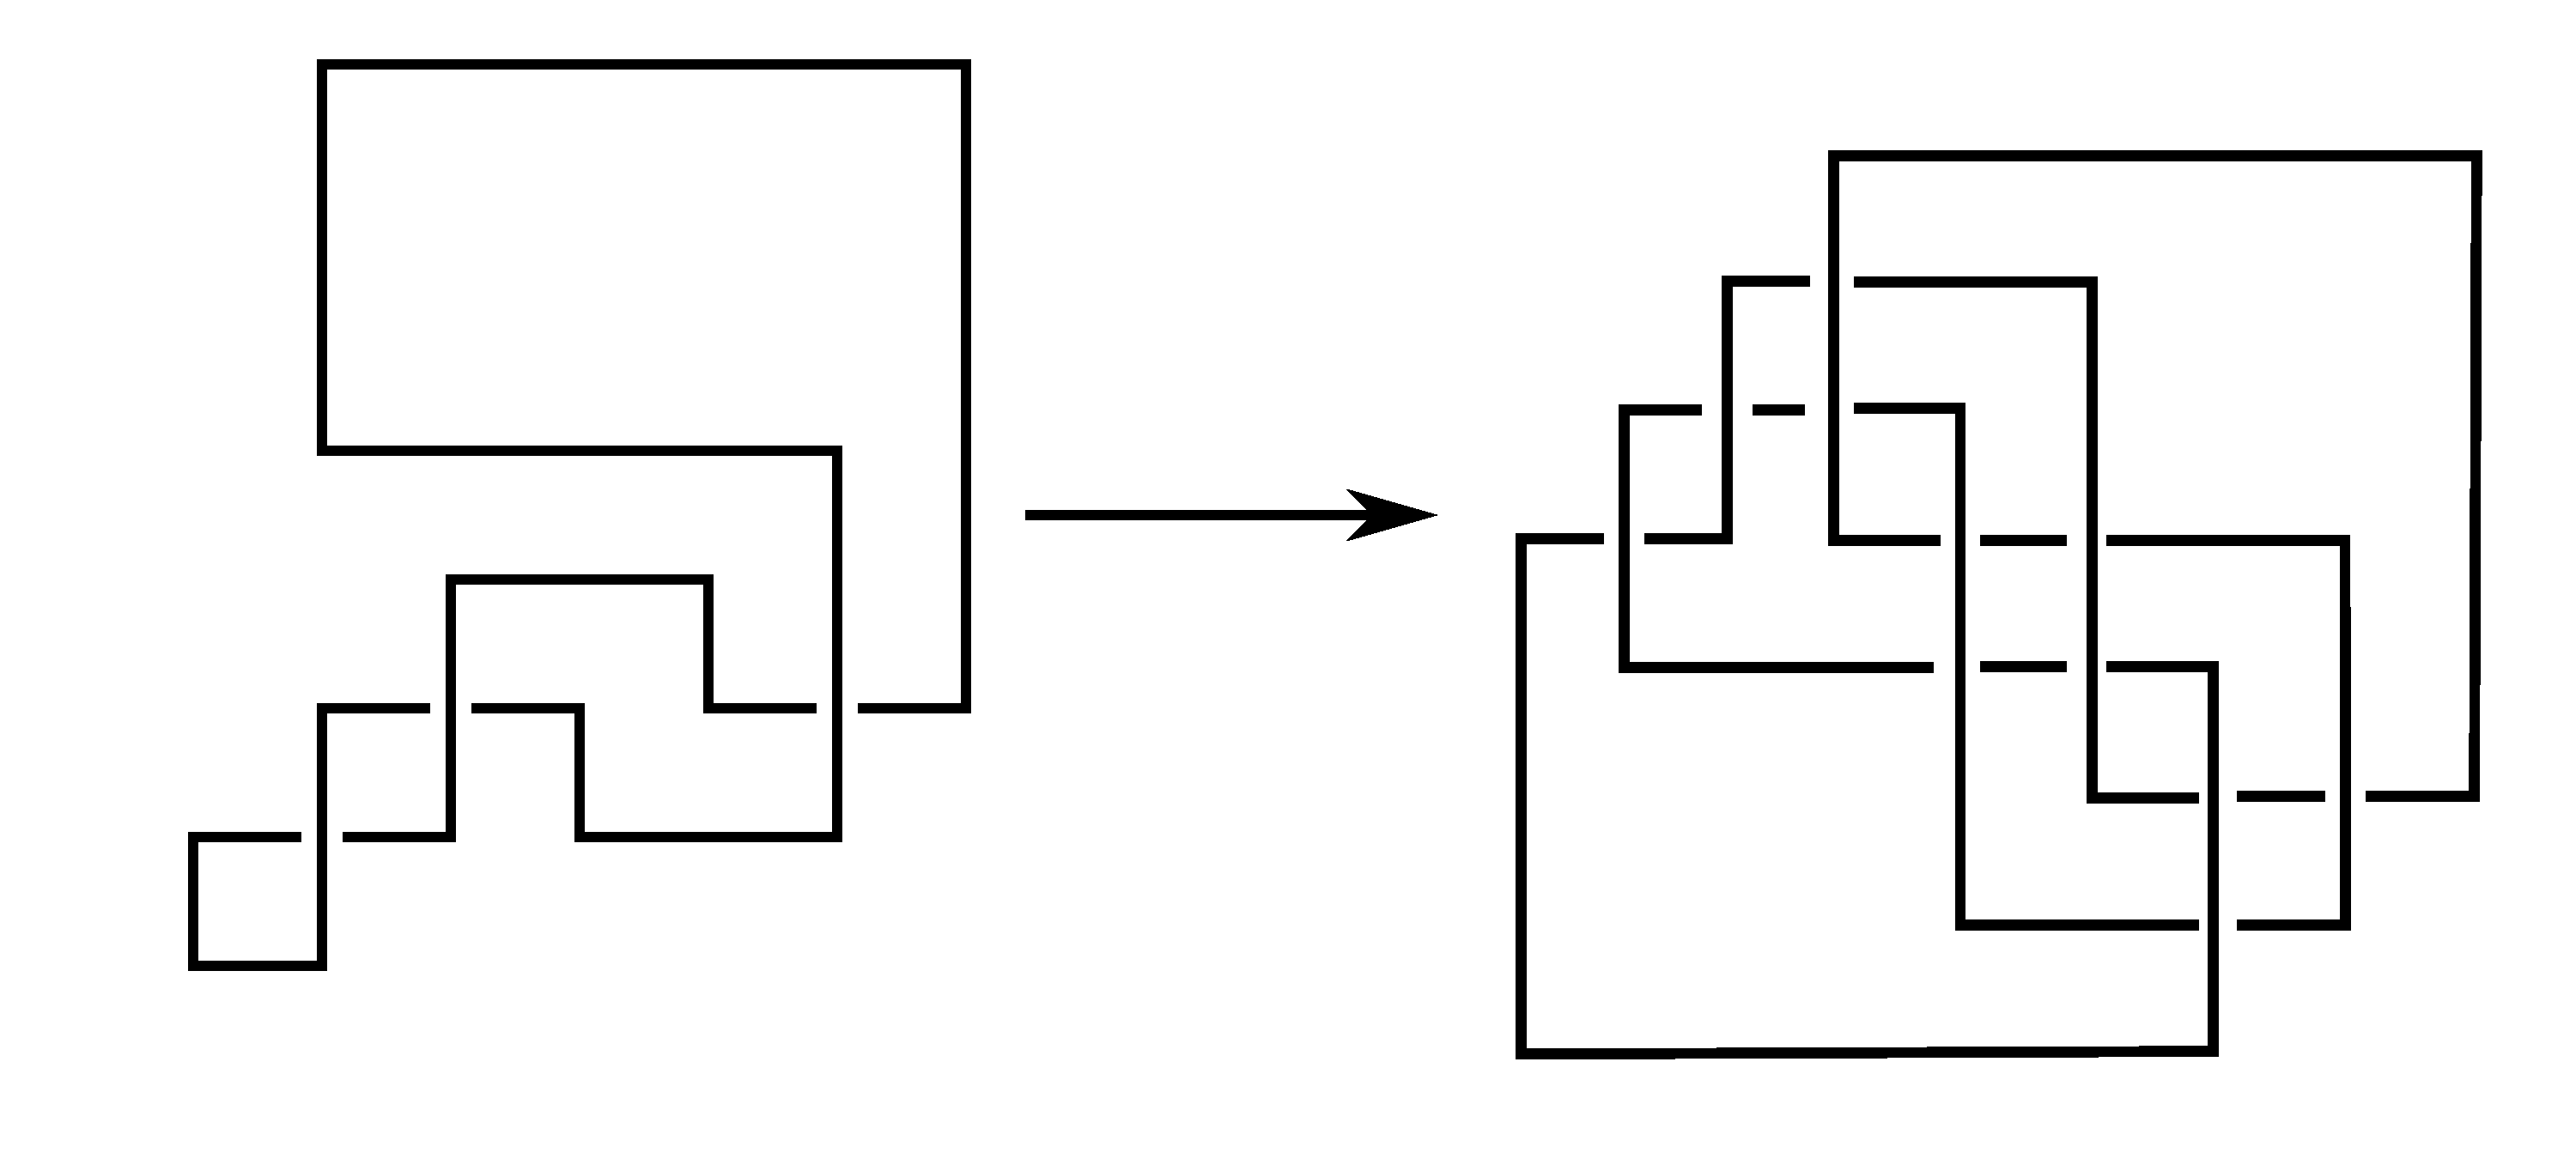
\includegraphics[width=0.4\textwidth]{images/pretzel-+4-construction.pdf}
            \label{fig:pretzel+4}
            \caption{Unknot and resulting diagram for $P_{4}$.}
        \end{figure}

\end{itemize}
